\subsubsection{Planar Budget Response Across Time}
\begin{figure*}[t]
\centering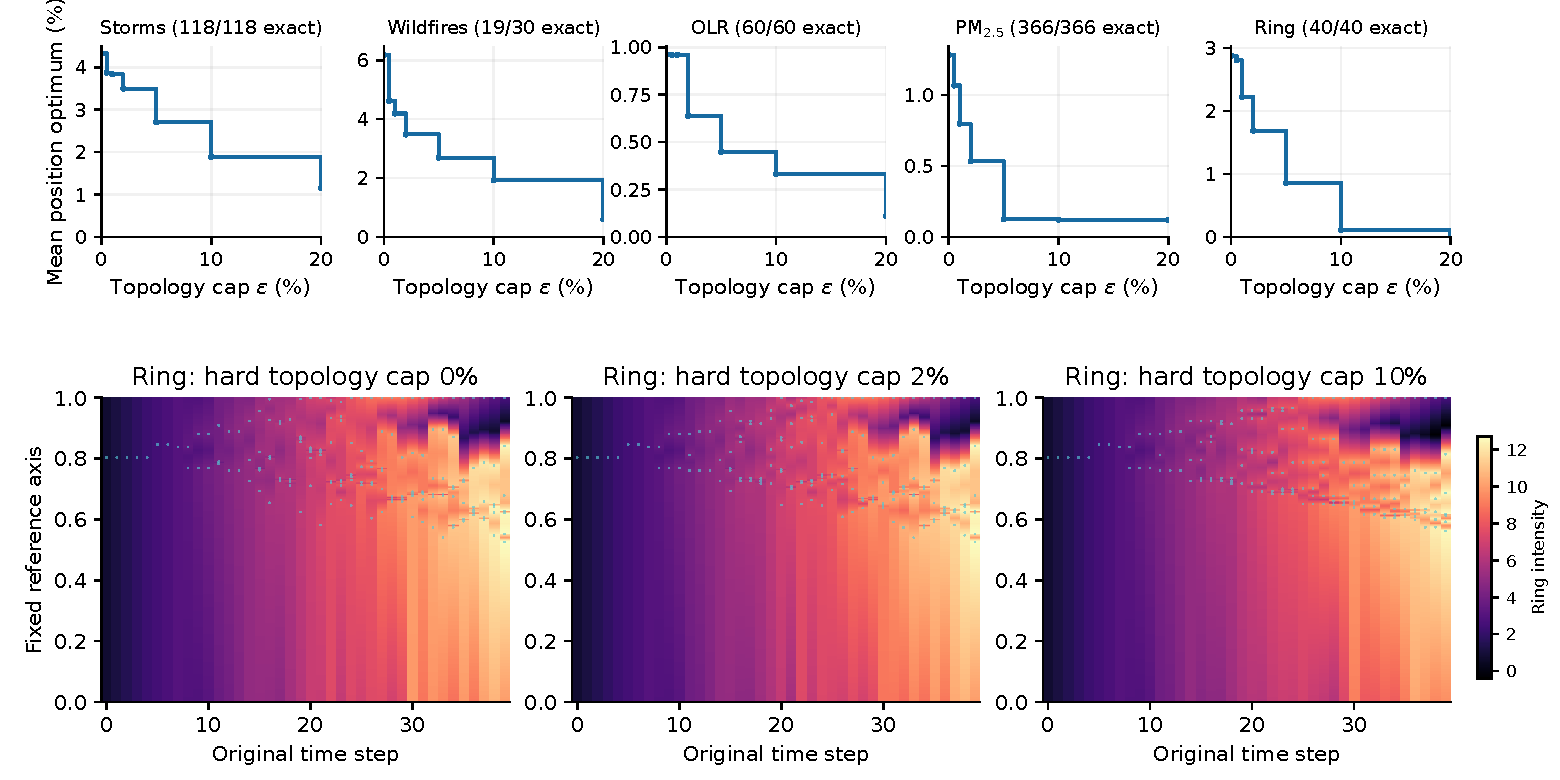
\includegraphics[width=\textwidth]{figures/Fig15.pdf}
\caption{New hard-budget family experiments. Top: temporal means of framewise minimax reference error against a true labelled topology-error cap; titles disclose exhaustive coverage. Wildfires includes 11 candidate-only upper bounds, using the same pool at every cap. Bottom: Ring scalar witness maps at 0\%, 2\% and 10\% topology allowances, with LP anchors in cyan and the same scalar colour scale. These piecewise-linear barrier witnesses illustrate changing admissible orders; they do not reconstruct source fields or establish temporal smoothness. The plotted rasters are illustrative; continuous saved anchors and barriers supply the budget checks.}
\label{fig:budget_response}
\end{figure*}
The threshold system changes which orders can be displayed, rather than merely changing a weighted objective. Small allowances retain expensive order conflicts; larger allowances admit additional orders until a frame reaches the free-packing regime or the best order in the declared candidate pool. The Ring maps illustrate the selected LP witnesses across the original 40 fields. Their framewise selection can change between columns; a smooth temporal solution requires an explicitly specified secondary policy within the budgets. The earlier R2/R20/R100 curves describe another construction policy, not these hard topology caps.
